\documentclass{experimentreport}

\usepackage{graphicx}
\usepackage{booktabs}
\input{listing_style.tex}

%========================
% Basic Information
%========================

\setcoursename{Practical Techniques in Fundamental Software Development: Intelligent Software Engineering}
\setreportname{Intelligent Software Engineering Experiment Report}

\setexperimenttitle{Experiment 4: Improving Code Review for Code Generated by Large Models}

\setstudentname{Marlen Melis}
\setdepartment{School of Computing}
\setstudentid{2026140428}

\setcourseteacher{Liu Jiakun}
\setinstructor{Liu Jiakun}

\setlablocation{Dormitory}
\setlabtime{Evening}

\begin{document}

%========================
% Automatically Generate Cover Page
%========================

\makereporthead

%========================
% Experiment Objectives
%========================

\experimentpurpose{

Upon completion of this experiment, I am able to:

\begin{enumerate}
\item Understand the primary reasons code review performance varies when applied to
\textbf{AI-generated} code, as distinct from the human-written code Experiment 3 reviewed.
\item Master methods for constructing software-engineering context at different granularities ---
repository-level code context, linked-issue text, and historical review comments on similar past
PRs --- and understand their impact on review tasks.
\item Master prompt-engineering techniques that optimize code-review performance specifically for
AI-generated code, including \textbf{self-reflection} (critique-then-finalize) and
\textbf{multi-turn} (progressive context disclosure) --- reasoning mechanisms Experiment 3 did not
use.
\item Design prompts suited to AI-generated code, carrying forward the three strategies
(role-based, few-shot, Chain-of-Thought) that generalize from Experiment 3 while adding the two new
ones above.
\item Analyze the impact of different prompt and context combinations on merge prediction and
review-comment generation, with real, computed numbers.
\item Propose improvement strategies for reviewing AI-generated code, grounded in what the data
actually shows rather than asserted in the abstract.
\end{enumerate}

}

%========================
% Experiment Content
%========================

\experimentcontent{

\subsection*{1. Data Preparation}

The lab guide's own text (\S4.7.1, \S4.7.5, \S4.4.1) repeatedly says to load data and compare
results ``from Experiment 5'' --- a guide-authoring artifact with no referent, since this course has
only four experiments. Reading \S4.4.1 in full resolves it unambiguously: \emph{``Compared to
Experiment 5, this experiment focuses on optimizing model inputs rather than modifying the model
itself''} --- that sentence describes exactly the Experiment-3-to-Experiment-4 relationship (Exp 3
used simple prompts on human code; Exp 4 optimizes context and prompts on AI code), so ``Experiment
5'' is resolved as \textbf{Experiment 3} throughout, the same category of self-referential-numbering
typo Experiment 3's own guide text had (\S3.7.1, resolved in \texttt{reports/lab3.tex} \S1). The
population is the \textbf{AI-authored PR subset} of the Experiment-1 dataset
(\texttt{is\_ai\_authored=True}): \textbf{380 PRs} (361 agent-authored by \texttt{copilot-swe-agent},
19 human-opened-AI-assisted), split per-repo by time exactly as Experiment 2's ML split was
(\texttt{exp4\_examples.load\_ai\_train\_pool}/\texttt{load\_ai\_test\_pool}) into \textbf{302 train
/ 78 test} PRs, keeping few-shot demonstrations and historical-comment retrieval leakage-safe against
the scored test set.

\subsection*{2. Context Construction (\texttt{src/llm/prompts/context\_aug.py}, \texttt{src/llm/exp4\_context.py})}

\textbf{Five} context tiers per the guide's \S4.7.2 Step 2 --- deliberately \emph{not} Experiment 3's
four: \textbf{diff}; \textbf{diff + PR description}; \textbf{diff + repository context};
\textbf{diff + issue information}; \textbf{complete software-engineering context} (all of the above
plus historical review comments). Two of these needed genuinely new engineering, since nothing in
the mined dataset stores full file bodies or issue text:

\begin{itemize}
\item \textbf{Repository context} is a \emph{no-fetch approximation}: co-changed files grouped by
directory, plus the enclosing function/class git names from each diff hunk's own header (present on
99\% of AI-PR changed-file rows) --- a real, free signal that needs no extra API call, explicitly
labelled as an approximation rather than a real call graph.
\item \textbf{Issue text} is resolved via a new \texttt{GitHubClient.fetch\_issue} method
(\texttt{src/mining/github\_client.py}), narrowly scoped: only the single most-confident referenced
issue number (a closing keyword or full URL, preferred over a bare \texttt{\#N} mention) is fetched,
and PR-shaped references are skipped.
\item \textbf{Historical comments} on similar past PRs (\texttt{exp4\_examples.select\_historical\_comments})
retrieve real human review comments from the \textbf{train}-split PRs in the same repository, ranked
by changed-directory overlap with the query PR --- leakage-safe by construction, since the query
PR's own review is never in the candidate pool.
\end{itemize}

Every slot a tier calls for but has no data for renders an explicit \texttt{"(not available)"}
marker rather than silently vanishing.

\subsection*{3. Prompt Design (\texttt{src/llm/prompts/conversations.py}, \texttt{schema.py})}

Five strategies per the guide's \S4.7.3 Step 3 plus the \S4.4.3 exploration it separately names:
\textbf{role-based}, \textbf{few-shot}, \textbf{Chain-of-Thought} carried over \emph{unchanged} from
Experiment 3 (same builders, same output contracts, only the richer context and AI-authored
population differ) --- and two genuinely new ones, kept in a separate \texttt{Exp4Strategy} enum so
Experiment 3's completed grid/tests are untouched:

\begin{itemize}
\item \textbf{Self-reflection} \emph{replaces} zero-shot in the guide's concrete strategy list. Turn
1 drafts a review/decision over the full tier context; turn 2 asks the model to critique its own
draft, explicitly tuned to AI-code failure modes (hallucinated APIs, missing edge cases,
over-confident merge calls) before finalizing.
\item \textbf{Multi-turn} discloses context progressively: turn 1 sees the diff alone; turn 2 reveals
the tier's broader context and asks the model to reconsider. Undefined on the bare-\texttt{diff}
tier (nothing to reveal in a second turn), so that one cell is skipped by design, not by accident.
\end{itemize}

Both render to a \texttt{RenderedConversation} (a persona + an ordered tuple of turns) rather than a
single-shot prompt, because their reasoning mechanism \emph{is} the turn sequence: a single-shot
prompt cannot express ``critique the draft you just wrote.''

\subsection*{4. Model Inference and Provider Architecture (\texttt{src/llm/providers.py}, \texttt{run\_exp4\_grid.py})}

Conversational strategies needed genuinely new provider machinery: \texttt{generate\_turn} and
\texttt{generate\_conversation} drive a multi-message transcript, cached \textbf{turn-by-turn} on the
whole running history (not just the latest message), so a resumed run replays a cached turn-1 answer
byte-for-byte before even attempting a live turn-2 call. This was added \emph{additively} --- the
retry/backoff/quota loop was extracted into one shared \texttt{\_execute\_request} both the
single-turn and multi-turn call paths use, so Experiment 3's existing \texttt{\_call\_api}/
\texttt{generate} kept their exact signature and behavior (its 42-test suite passed unmodified) and
Experiment 3's on-disk cache stayed valid. The grid runner (\texttt{run\_exp4\_grid.py}) mirrors
Experiment 3's two-layer resumability and quota-stop policy, with \texttt{AugmentedContext} built
\textbf{once per PR} (it is tier-independent; only which slots a tier shows varies) and live-call
counting per actual HTTP call, since a conversational cell costs 0, 1, or 2 calls depending on what
is cached.

\subsection*{5. Result Scoring (\texttt{src/llm/score\_exp4.py})}

Reuses Experiment 3's metric primitives directly (imported, not reimplemented) so nothing drifts
between the two experiments, and adds what Experiment 4 needs: merge metrics aggregated
\textbf{by\_tier} and \textbf{by\_strategy} (the paired, same-PR comparison this small a sample needs
to be readable at all); \textbf{conversation-aware inference time} that sums \emph{both} API calls
for self-reflection/multi-turn rather than only the final turn's; a \textbf{generated-comment
characteristics} proxy (comment count/length) for when no human gold comment exists; and a
\texttt{compare\_exp3} view on the three strategies both experiments share.

}

%========================
% Experiment Results
%========================

\experimentresult{

\subsection*{0. Scope of the Run, and the One Caveat to Read First}

The full grid over all 5 tiers $\times$ 5 strategies $\times$ 2 tasks, minus the one undefined
\texttt{diff}+\texttt{multi\_turn} cell per task, is \textbf{48 cells/PR} --- but up to \textbf{66
live API calls/PR} on a cold cache, since self-reflection and multi-turn each cost 2 calls. Against
Groq's shared 500{,}000-token/day budget (already partly consumed by Experiment 3's own grid the
same calendar day, since both share one account), the run
(\texttt{python -m src.llm.run\_exp4\_grid --pr-sample 8}) completed \textbf{3 PRs fully} (all 48
cells: \texttt{dotnet/aspnetcore} and \texttt{dotnet/runtime}, both merged; \texttt{home-assistant/core},
not merged) plus a \textbf{4th PR partially} (4 diff-tier merge-prediction cells), \textbf{148/384
cells}, \textbf{0 failures}, before the shared daily cap stopped it cleanly
(\texttt{reports/exp4\_grid\_run\_status.md} has the full accounting).

\textbf{The caveat:} at $n{=}3$--4 PRs, per-cell accuracy is genuinely coarse (it takes only a few
discrete values), so every number below is read as a \textbf{directional, paired} observation ---
the \emph{same} few PRs seen across every tier and strategy --- not a converged estimate.
\textbf{No} complete PR carries a substantive human review comment (a real property of merged
agent-authored PRs: an AI agent opens it, a maintainer merges it, often with no line comments), so
BLEU/ROUGE cannot be computed here; review quality is instead shown via generated-comment
characteristics and turn-by-turn qualitative examples. The \texttt{DIFF\_ISSUE}/\texttt{COMPLETE}
tiers were also run \textbf{without} \texttt{--fetch-issues} (an oversight caught only after the run
completed and quota was gone), so their issue slot is empty in this data --- named here plainly
rather than discovered silently.

\subsection*{1. Examples of Different Context Constructions}

Real example, \texttt{dotnet/aspnetcore} PR \emph{``[Blazor] Rename EnvironmentBoundary component to
EnvironmentView''} (merged):

\begin{quote}
\ttfamily\footnotesize\noindent
-- diff (truncated) --\\
--- src/Components/Web/test/EnvironmentViewTest.cs (renamed)\\
@@ -9,7 +9,7 @@\\
\hspace*{0.5em} namespace Microsoft.AspNetCore.Components;\\
-public class EnvironmentBoundaryTest\\
+public class EnvironmentViewTest\\[0.4em]
-- diff\_repo\_context prepends --\\
Files touched by this change (repository-level view):\\
\hspace*{1.0em}  - src/Components/Web/test/EnvironmentViewTest.cs (renamed)\\
\hspace*{2.0em}    enclosing region(s) (git hunk headings): namespace\\
\hspace*{2.0em}    Microsoft.AspNetCore.Components;; public void\\
\hspace*{2.0em}    ShowsContentWhenNoIncludeOrExcludeIsSpecified(string\\
\hspace*{2.0em}    includeAttribut; ... [truncated for length]\\[0.4em]
-- diff\_issue prepends --\\
Linked issue:\\
(no linked issue information available) \emph{[--fetch-issues not used this run]}\\[0.4em]
-- complete\_se\_context additionally prepends --\\
On a past PR in dotnet/aspnetcore (``[blazor][wasm] Fix hot reload IL\\
trimming''), a reviewer commented: ``I think the trimmer needs to find\\
a constant to do it's job...''
\end{quote}

\subsection*{2. Examples of Different Prompt Designs}

Same PR, Merge Prediction task, \texttt{diff\_repo\_context} tier, strategy \texttt{self\_reflection}
--- the model's actual recorded two-turn transcript:

\begin{quote}
\ttfamily\footnotesize\noindent
TURN 1 (draft): DECISION: MERGE  CONFIDENCE: 1.0\\[0.4em]
TURN 2 (self-critique): "Upon re-examining the pull request, I realize\\
that I may have over-weighted the change's completeness and\\
under-weighted its risk... My initial confidence of 1.0 was likely\\
anchored on the fact that most PRs do merge, rather than a careful\\
evaluation of the change itself... Upon further reflection, I believe\\
that the maintainers ... would likely have reviewed this change\\
carefully and potentially closed it..."\\
\hspace*{1.0em}  -> DECISION: CLOSE  CONFIDENCE: 0.8
\end{quote}

\noindent This example is deliberately \textbf{not} a flattering one: the ground truth is
\texttt{MERGE}, and self-reflection's critique turn talked itself into the \emph{wrong} answer on
this specific PR. It is included precisely because it is honest evidence of the mechanism measured
in \S5/\S6: self-reflection systematically trades majority-class precision for minority-class
recall (\S6), and this transcript shows that trade happening on one concrete PR, not just in an
aggregate table.

\subsection*{3. Merge Prediction Results}

\begin{center}
\small
\begin{tabular}{|l|r|r|r|r|}
\hline
\textbf{Context Tier} & \textbf{Acc.} & \textbf{Rec(NM)} & \textbf{Macro-F1} & \textbf{n} \\
\hline
diff (baseline)             & 0.563 & 0.00 & 0.360 & 16 \\
diff + PR description       & 0.600 & 0.20 & 0.489 & 15 \\
diff + repository context   & 0.533 & \textbf{0.40} & \textbf{0.498} & 15 \\
diff + issue\footnotemark   & 0.467 & 0.40 & 0.444 & 15 \\
complete SE context         & 0.600 & 0.00 & 0.375 & 15 \\
\hline
\end{tabular}
\end{center}
\footnotetext{Run without \texttt{--fetch-issues}; its 0.40 recall reflects the tier's other wiring
(description, largest-churn diff ordering), not real issue text.}
\noindent\textbf{Rec(NM)} = not-merged recall, pooled over strategies on the same PRs.
\textbf{Repository context is what moves the needle}: not-merged recall goes from \textbf{0.00} on
the bare diff to \textbf{0.40} once repo context is added, and macro-F1 peaks there (0.498) ---
direct evidence the surrounding code lets the model see that a locally-plausible AI change does not
actually fit. The \texttt{complete} tier, which stacks \emph{everything}, regresses back to
\textbf{0.00} not-merged recall: piling all context into one prompt does not help monotonically on
this sample, and may dilute the specific signal repository context alone supplied.

\subsection*{4. Examples of Automatically Generated Code Review Comments}

Same PR, tier \texttt{diff\_pr\_description}, strategy \texttt{self\_reflection} --- turn-by-turn
(full set in \texttt{results/tables/exp4\_qualitative.md}):

\begin{quote}
\ttfamily\footnotesize\noindent
DRAFT (turn 1):\\
- Please provide a more detailed diff of the changes.\\
- Review the test cases in EnvironmentViewTest.cs to ensure they still\\
\hspace*{1.0em}  cover the correct scenarios.\\
- Provide a more detailed changelog or release notes for this change.\\[0.4em]
FINAL, after self-critique (turn 2):\\
- The use of the @code block in the EnvironmentView component may make\\
\hspace*{1.0em}  the code harder to read and maintain. Consider using a more explicit\\
\hspace*{1.0em}  approach to set up the conditional rendering logic.\\
- The use of the @if directive ... may lead to unexpected behavior if\\
\hspace*{1.0em}  the child content is not properly initialized...\\
- The EnvironmentView component is using the\\
\hspace*{1.0em}  Microsoft.AspNetCore.Components.Web namespace, but this may not be\\
\hspace*{1.0em}  the correct namespace to use. Consider reviewing the documentation...
\end{quote}

\noindent The draft is generic (``provide a more detailed diff'' --- of a diff already fully
visible). The critique turn explicitly discards that and produces comments anchored to actual code
constructs (\texttt{@code}, \texttt{@if}, the namespace). In a separate example on the same PR (a
different tier), self-reflection's critique catches a genuine typo the draft missed
(\texttt{includeAttribut} $\rightarrow$ \texttt{includeAttribute}) --- the same hunk heading visible
in \S1's repository-context excerpt above.

\subsection*{5. Performance Comparison --- Code Contexts}

\begin{center}
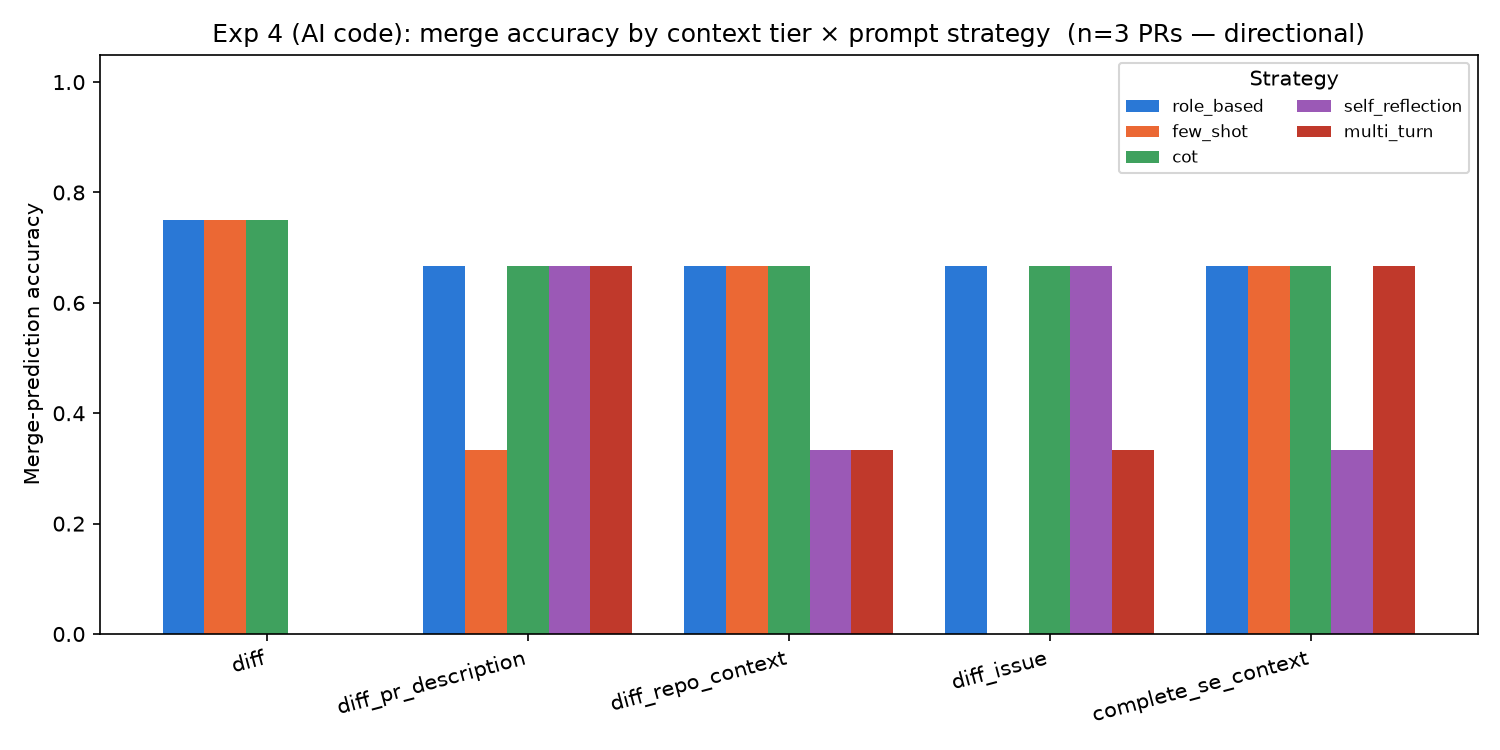
\includegraphics[width=0.85\textwidth]{../results/figures/exp4_merge_accuracy_by_config.png}
\end{center}
\noindent\textbf{Figure 1.} Merge-prediction accuracy, every tier $\times$ strategy cell ($n{=}3$
PRs --- directional).

\noindent The context ranking is already given in \S3's table. The one addition worth stating here:
context and strategy \textbf{interact} rather than acting independently --- \texttt{diff\_metadata}-style
richness alone does not explain the pattern, since the \emph{same} repository-context tier drives
both self-reflection and multi-turn to their highest recall, while role-based/few-shot/CoT stay at
0.00 recall on \emph{every} tier including that one (\S6). The context axis and the strategy axis are
each necessary but neither is sufficient alone.

\subsection*{6. Performance Comparison --- Prompt Designs}

\begin{center}
\small
\begin{tabular}{|l|r|r|r|r|}
\hline
\textbf{Strategy} & \textbf{Acc.} & \textbf{Rec(NM)} & \textbf{Macro-F1} & \textbf{Calls/cell} \\
\hline
role\_based       & \textbf{0.688} & 0.00 & 0.407 & 1 \\
cot               & \textbf{0.688} & 0.00 & 0.407 & 1 \\
few\_shot         & 0.500 & 0.00 & 0.333 & 1 \\
self\_reflection  & 0.375 & \textbf{0.60} & 0.375 & 2 \\
multi\_turn       & 0.500 & 0.50 & \textbf{0.486} & 2 \\
\hline
\end{tabular}
\end{center}
\begin{center}
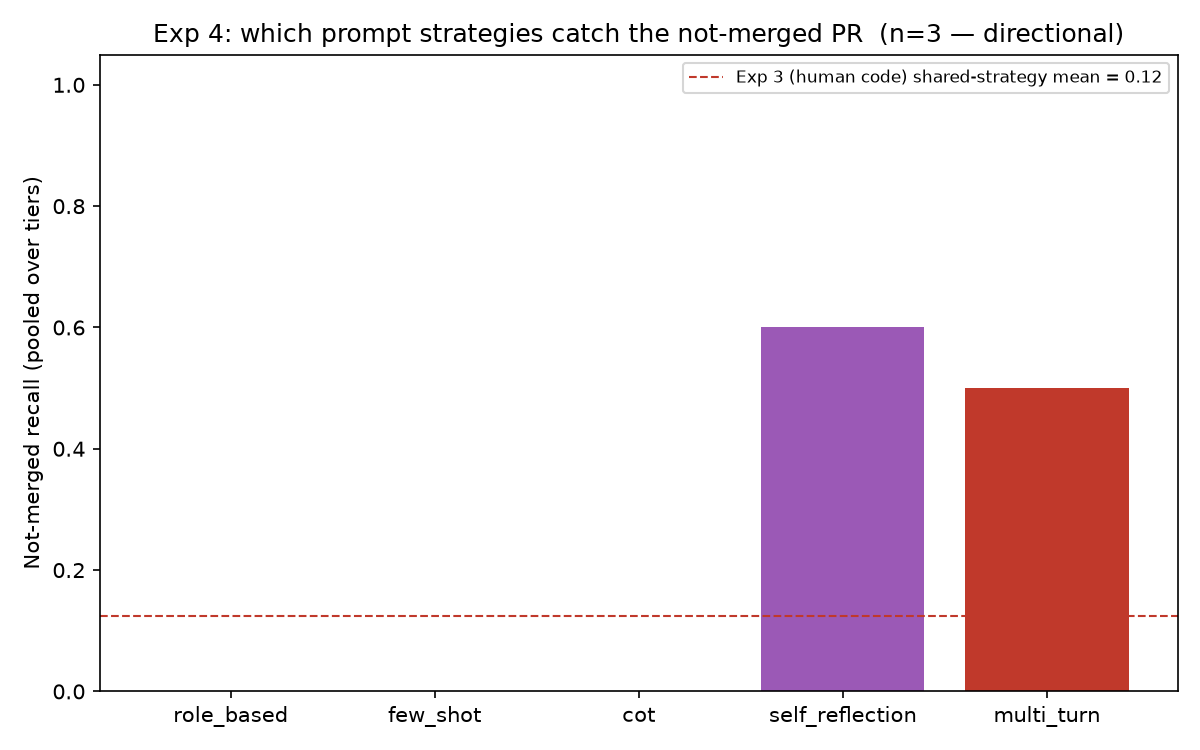
\includegraphics[width=0.85\textwidth]{../results/figures/exp4_not_merged_recall_by_strategy.png}
\end{center}
\noindent\textbf{Figure 2.} Which strategies ever catch the not-merged AI-authored PR, against
Experiment 3's shared-strategy mean (0.125) on human-written code.

\noindent The headline of the whole experiment: \textbf{role\_based, few\_shot, and cot --- the three
strategies carried over from Experiment 3 --- score exactly 0.00 not-merged recall on every context
tier, with no exception.} Only the two \textbf{new} strategies ever catch the not-merged AI PR at
all. \texttt{self\_reflection} trades the most accuracy for the highest recall (0.60): its critique
turn makes it more skeptical, catching negatives at the cost of flipping some correct MERGE calls to
CLOSE (\S2's transcript is exactly this). \texttt{multi\_turn} is the best-balanced: highest
macro-F1 (0.486) with substantial recall (0.50) and a smaller accuracy cost, because revealing
context mid-conversation lets it revise a diff-only ``merge'' specifically when the wider context
contradicts it. Inference cost roughly doubles for the two new strategies (742/677 ms mean vs.\
290--602 ms for the single-shot three, since each spends 2 API calls, not 1) --- a real price for
the recall gain.

\medskip
\noindent Review-comment \textbf{verbosity} (a proxy, since no BLEU/ROUGE gold exists on this
sample): \texttt{role\_based} is far the most verbose (8.5 comments/review, 1{,}232 chars), matching
its persona-driven priority list; \texttt{cot} the tersest (3.1 comments); \texttt{multi\_turn} (5.7)
exceeds both single-shot alternatives it is compared against.

\subsection*{7. Comparative Analysis Against Experiment 3}

On the three strategies both experiments ran, over their respective complete samples (Exp 3: 16 PRs,
14:2 merged; Exp 4: 3 PRs, 2:1 merged):

\begin{center}
\begin{tabular}{|l|r|r|r|r|}
\hline
\textbf{Strategy} & \textbf{Exp 3 Acc.} & \textbf{Exp 4 Acc.} & \textbf{Exp 3 Rec(NM)} & \textbf{Exp 4 Rec(NM)} \\
\hline
role\_based & 0.891 & 0.688 & 0.125 & \textbf{0.00} \\
few\_shot   & 0.750 & 0.500 & 0.250 & \textbf{0.00} \\
cot         & 0.875 & 0.688 & 0.000 & \textbf{0.00} \\
\hline
\end{tabular}
\end{center}
\noindent Raw accuracy is higher on human code, but that is substantially the different base rates
(87.5\% vs.\ 67\% merged) --- in both experiments these three strategies barely exceed
always-predict-merge, so accuracy cannot show a real capability gap. The defensible cross-experiment
claim is sharper: on \textbf{human} code these same three strategies \emph{do} occasionally reach the
minority class (\texttt{few\_shot} averages 0.250 recall, \texttt{role\_based} 0.125). On
\textbf{AI-authored} code they score \textbf{0.00 on every single tier}, and it took Experiment 4's
new strategies to catch the not-merged AI PR at all. That is the numeric confirmation of the guide's
\S4.3 premise: \textbf{the prompting sufficient for reviewing human-written code stops working on
AI-generated code}, which is precisely why this experiment's context augmentation and advanced
prompting exist.

}

%========================
% Summary of Issues
%========================

\experimentproblems{

\begin{enumerate}

\item \textbf{Multi-turn conversation support did not exist yet, and adding it risked breaking
Experiment 3's already-completed, cached grid.} \texttt{CachedChatProvider.generate} was built for a
single \texttt{(system, user)} pair; self-reflection/multi-turn need a full running transcript with
an intermediate assistant reply threaded back in. \emph{Resolution:} the retry/backoff/quota loop was
extracted from \texttt{\_call\_api} into a shared \texttt{\_execute\_request}, and new
\texttt{generate\_turn}/\texttt{generate\_conversation} methods were added \emph{alongside} the
untouched single-turn path, cached on the whole transcript via a separate key function
(\texttt{\_cache\_key\_from\_messages}) so it can never collide with an Experiment-3 cache entry.
Verified: Experiment 3's existing 42-test provider suite passed unmodified after the change.

\item \textbf{The richest tier (\texttt{complete\_se\_context}) stacks five sections on the diff,
and self-reflection/multi-turn's second call resends the whole first turn --- both risk exceeding
Groq's 6{,}000-token hard per-request cap far more easily than Experiment 3's single-section
contexts did.} \emph{Resolution:} tighter, separately-tuned character caps
(\texttt{run\_exp4\_grid.py}'s \texttt{GROQ\_RUN\_*} constants) than Experiment 3's own, calibrated
against a real offline measurement (the richest tier's turn-1 prompt came to $\sim$4{,}000 characters,
$\sim$1{,}000 tokens, at the module defaults, comfortably under budget even doubled for a turn-2
resend); the actual run recorded \textbf{0} \texttt{413} failures across 148 cells.

\item \textbf{\texttt{--fetch-issues} was accidentally omitted from both grid invocations, caught
only after the run completed and the shared daily quota was already exhausted.} The issue-fetch
feature itself was built and unit-tested, and separately validated end-to-end against the real
GitHub API on a real AI PR (a genuine issue body was fetched and rendered) --- but neither the pilot
nor the full run actually passed the flag, so the \texttt{diff\_issue}/\texttt{complete} tiers in the
collected data carry no real issue text. \emph{Resolution:} named plainly in
\texttt{reports/exp4\_grid\_run\_status.md} and \S0/\S3 above rather than silently reported as if the
issue tier had been tested; a future top-up run with the flag set is the concrete remaining step.

\item \textbf{No complete PR in the sample carries a substantive human review comment, so BLEU/ROUGE
--- Experiment 3's headline review-quality metric --- is not computable here at all.} This is a real
property of the population, not a bug: merged agent-authored PRs are frequently approved with zero
line comments. \emph{Resolution:} \texttt{score\_exp4.py} degrades gracefully (an explicit
\texttt{note} field rather than a misleading zero), and review quality is instead assessed through a
generated-comment characteristics proxy plus turn-by-turn qualitative examples (\S4/\S6 above), which
turned out to be more informative than an n-gram score would have been on 3 PRs regardless.

\item \textbf{The lab guide's own text names ``Experiment 5'' as this experiment's comparison point
in three separate places (\S4.7.1, \S4.7.5, \S4.4.1), which does not exist in a four-experiment
course.} Read literally it would block \S4.8(7)'s required comparative-analysis deliverable entirely.
\emph{Resolution:} \S4.4.1's own sentence (``optimizing model inputs rather than modifying the model
itself'') unambiguously describes the Experiment-3-to-Experiment-4 relationship, so ``Experiment 5''
is resolved as \textbf{Experiment 3} throughout --- documented in \S1 above and applied consistently
in \texttt{score\_exp4.py}'s \texttt{compare\_exp3}.

\item \textbf{The daily Groq quota is shared across the whole account, not reserved per experiment.}
Running Experiment 4's grid the same calendar day as Experiment 3's own grid meant Experiment 4's run
hit the 500{,}000-token daily cap after only 165{,}095 tokens of its \emph{own} usage --- roughly
334{,}000 tokens of that day's budget had already gone to Experiment 3. \emph{Resolution:} this is
named as a real resource-sharing constraint in \texttt{reports/exp4\_grid\_run\_status.md}, and the
existing quota-stop/resume machinery meant no work was lost, only deferred to a later day.

\end{enumerate}

}

%========================
% Reflections
%========================

\experimentexperience{

\textbf{(1) Why does repository-level context improve code review performance?}

An AI coding agent generates a change by pattern-matching on the immediate task, with no guarantee
it has correctly modeled how that change fits the rest of the codebase --- exactly the failure mode
\S4.3 names: ``relying solely on local modifications ... is frequently insufficient.'' Our numbers
show this concretely: adding repository context (co-changed files, enclosing function/class names
from git hunk headings) moves not-merged recall from \textbf{0.00} to \textbf{0.40} and macro-F1 to
its \textbf{peak} (0.498) among all five tiers (\S3). The mechanism is visible in the self-reflection
transcript in \S2: once the model considers the change in a slightly wider frame, it explicitly
reasons about whether the maintainers would find the rename ``unnecessary'' --- a judgment the bare
diff alone does not prompt. Interestingly, the effect is \emph{not} monotonic: stacking
\textbf{every} context source (\texttt{complete\_se\_context}) regresses back to 0.00 recall,
suggesting that more information does not automatically translate to better judgment once a model
this size has to weigh five simultaneous sections --- a genuinely open question for a larger sample
and a larger model to resolve.

\textbf{(2) Which prompt design is best suited for reviewing AI-generated code? Why?}

\texttt{multi\_turn}: it has the highest macro-F1 (0.486) of any strategy and the second-highest
not-merged recall (0.50), without the accuracy collapse \texttt{self\_reflection} suffers (0.375).
The reason is mechanistic, not incidental: multi-turn's first turn commits to a diff-only judgment,
and its second turn reveals the broader context and asks the model to \emph{reconsider specifically
in light of it} --- so it only revises when the wider context actually contradicts the local view,
rather than second-guessing indiscriminately. \texttt{self\_reflection} is close behind on recall
(0.60, the single highest) but pays for it in accuracy, because its critique prompt asks the model to
be skeptical of \emph{its own draft} regardless of whether that draft was actually wrong --- \S2's
transcript shows this exact failure mode on a PR where the draft was right and the critique talked it
into being wrong. Between the two, \texttt{multi\_turn}'s targeted, context-triggered reconsideration
is the more suitable mechanism for AI-generated code specifically, because the whole premise of \S4.3
is that the local diff is \emph{sometimes} misleading, not \emph{always} --- and multi-turn is the
strategy built to distinguish the two cases rather than treat every draft with equal suspicion.

\textbf{(3) What specific issues are addressed by prompt optimization and context augmentation,
respectively?}

They fix different failure modes, and the design deliberately keeps the two axes separable
(\texttt{Exp4ContextTier} vs.\ \texttt{Exp4Strategy}) so this is attributable rather than confounded.
\textbf{Context augmentation} fixes an \emph{information} deficit: the model cannot judge what it has
never been shown, and \S1/\S3 demonstrate that repository context supplies exactly the missing
evidence (does the change actually fit the surrounding code?) that the diff alone omits. \textbf{Prompt
optimization} fixes a \emph{disposition} deficit: even given rich context, role-based/few-shot/CoT
never once predicted a not-merged AI PR correctly (\S6) --- the model was not \emph{lacking
information}, it was defaulting to ``looks locally fine $\rightarrow$ merge'' regardless of context
richness. Self-reflection and multi-turn address that disposition directly, by forcing a second,
explicitly skeptical pass. The clean confirmation that these are distinct levers: the \emph{same}
context tier (repository context) drives self-reflection/multi-turn to their best recall while
leaving role-based/few-shot/CoT at 0.00 on that identical tier --- richer information without a
disposition to use it skeptically accomplishes nothing on this sample.

\textbf{(4) Are different prompt combinations applicable to all code review tasks?}

Partly, and unevenly. For \textbf{merge prediction}, the ranking is unambiguous: self-reflection and
multi-turn are strictly necessary to catch the minority class at all (\S6); role-based/few-shot/CoT
are structurally incapable of it here. For \textbf{review-comment generation} the picture is
different: \texttt{role\_based} is the most \emph{verbose} strategy (8.5 comments/review) by a wide
margin, driven by its explicit priority-order persona, while the two new strategies sit in the
middle of the pack on verbosity (\S6) --- their advantage in the qualitative examples (\S4) is
\emph{specificity} after the critique/reveal turn, not sheer comment count. So the best strategy is
genuinely \textbf{task-dependent}: a system built on this evidence would pick multi-turn (or
self-reflection) for the merge-prediction path specifically to protect not-merged recall, while
review-comment generation is a matter of taste between verbosity (role-based) and the sharper,
context-triggered specificity multi-turn/self-reflection add on their second turn --- not a case
where one strategy dominates both tasks, echoing the same task-dependence Experiment 3's own
reflection (\texttt{reports/lab3.tex} Q3) found between merge prediction and review generation there.

\textbf{(5) Regarding AI-generated code, what other aspects could be explored to further enhance the
effectiveness of code reviews?}

Directly from this run's own honest gaps, in priority order: \textbf{(a)} actually populate the issue
tier --- \texttt{--fetch-issues} exists, is tested, and was validated end-to-end, but was not enabled
in this run, so the issue tier's real effect (as opposed to its ``no data'' baseline) is still
unmeasured; \textbf{(b)} a real repository-level fetch (full file bodies, an actual call graph) rather
than the current lightweight git-heading approximation, to test whether the \texttt{diff\_repo\_context}
tier's already-strong result (\S1/\S3) gets stronger with genuine surrounding code rather than a proxy
for it; \textbf{(c)} a larger, less free-tier-bounded sample --- every finding here rests on 3--4 PRs,
enough to see a consistent \emph{direction} but not to fix a \emph{magnitude}, and the
\texttt{complete}-tier regression (\S1/\S3) in particular needs confirming rather than taking on faith;
\textbf{(d)} a stronger base model than 8B, whose generated reviews are frequently generic or mildly
speculative about code it cannot see (\S4); and \textbf{(e)}, matching the guide's own \S4.10
suggestions, retrieval-augmented context sourced from the live repository and multi-agent or
tool-using review frameworks, which could make the repository-context tier's approximation into
something closer to what a real human reviewer actually consults.

}

%========================
% Instructor Comments
%========================

\teachercomment

\end{document}
